\documentclass[11pt]{article}
\usepackage[utf8]{inputenc}
\usepackage[margin=1in]{geometry}
\usepackage[titletoc,title]{appendix}
\usepackage{fancyhdr}
\usepackage[T1]{fontenc}
\usepackage{bm}
\usepackage{courier}
\usepackage[colorlinks = true,linkcolor = blue]{hyperref}
\usepackage{amsmath,amsthm,amsfonts,amssymb,mathtools}
\newcommand{\bmat}[1]{\begin{bmatrix}#1\end{bmatrix}}
\newcommand{\norm}[2][]{\lVert#2\rVert_{#1}}
\DeclareMathOperator{\tr}{tr}
\usepackage{graphicx,float}
\usepackage{minted}
\newminted{python}{frame=lines,framesep=2mm,baselinestretch=1.1,linenos}
\usepackage{subcaption}
\usepackage{changepage}

\pagestyle{fancy} \fancyhf{}
\lhead{Homework 4} \rhead{AI501}
\rfoot{\thepage}
\title{Homework 4}
\author{20213073 Donggyu Kim}
\date{May 24, 2021}

\begin{document}
\maketitle
\thispagestyle{fancy}

\section{Equation}
Since $\bm\pi$ is under the constraint $\sum_{j=1}^{k}\pi_{j}=1$, we introduce the Lagrangian multiplier,
\begin{align*}
\tilde{\mathcal{L}}(\bm\theta,\lambda)
&=\tilde{\mathcal{L}}(\theta)+\lambda\left(1-\sum_{j=1}^{k}\pi_{j}\right) \\
&=\sum_{i=1}^{n}\sum_{j=1}^{k}r_{i,j}^{(t)}(\log\pi_{j}+\log\mathcal{N}(\bm x_{i};\bm\mu_{j},\bm\Sigma_{j}))+\lambda\left(1-\sum_{j=1}^{k}\pi_{j}\right)
\end{align*}
We take the gradient w.r.t. $\bm\pi$ and get
\begin{align*}
\frac{\partial\tilde{\mathcal{L}}(\bm\theta,\lambda)}{\partial\pi_{j}}
=\sum_{i=1}^{n}\frac{r_{i,j}^{(t)}}{\pi_{j}}-\lambda=0\ \Rightarrow\ \pi_{j}^{(t)}
&=\frac{1}{\lambda}\sum_{i=1}^{n}r_{i,j}^{(t)}
\end{align*}
Using the constraint $\sum_{j=1}^{k}\pi_{j}=1$ again, we finally have
\begin{align*}
\sum_{j=1}^{k}\pi_{j}^{(t)}
&=\frac{1}{\lambda}\sum_{j=1}^{k}\sum_{i=1}^{n}r_{i,j}^{(t)} \\
&=\frac{1}{\lambda}\sum_{i=1}^{n}\sum_{j=1}^{k}\frac{\pi_{j}\mathcal{N}(\bm x_{i};\bm\mu_{j}^{(t-1)},\bm\Sigma_{j}^{(t-1)})}{\sum_{l=1}^{k}\pi_{l}\mathcal{N}(\bm x_{i};\bm\mu_{l}^{(t-1)},\bm\Sigma_{l}^{(t-1)})} \\
&=\frac{1}{\lambda}\sum_{i=1}^{n}1=\frac{n}{\lambda}=1\ \Rightarrow\ \lambda=n \\
\therefore\pi_{j}^{(t)} &= \frac{1}{n}\sum_{i=1}^{n}r_{i,j}^{(t)}
\end{align*}

By taking the gradient w.r.t. $\bm\mu$, we get
\begin{align*}
\frac{\partial\tilde{\mathcal{L}}(\bm\theta,\lambda)}{\partial\bm\mu_{j}}
&=\sum_{i=1}^{n}r_{i,j}^{(t)}\frac{\partial}{\partial\bm\mu_{j}}\left(-\frac{1}{2}(\bm x_{i}-\bm\mu_{j})^{\top}\bm\Sigma_{j}^{-1}(\bm x_{i}-\bm\mu_{j})\right) \\
&=\sum_{i=1}^{n}r_{i,j}^{(t)}(\bm x_{i}-\bm\mu_{j})^{\top}\bm\Sigma_{j}^{-1}=\bm 0 \qquad (\because\bm\Sigma_{j}=\bm\Sigma_{j}^{\top}) \\
\therefore\bm\mu_{j}^{(t)}&=\frac{1}{\sum_{i=1}^{n}r_{i,j}^{(t)}}\sum_{i=1}^{n}r_{i,j}^{(t)}\bm x_{i}
\end{align*}

This time, taking the gradient w.r.t. $\bm\Sigma^{-1}$, we get
\begin{align*}
\frac{\partial\tilde{\mathcal{L}}(\bm\theta,\lambda)}{\partial\bm\Sigma_{j}^{-1}}
&=\sum_{i=1}^{n}r_{i,j}^{(t)}\frac{\partial}{\partial\bm\Sigma_{j}^{-1}}\left(\frac{1}{2}\log(\det(\bm\Sigma_{j}^{-1}))-\frac{1}{2}(\bm x_{i}-\bm\mu_{j})^{\top}\bm\Sigma_{j}^{-1}(\bm x_{i}-\bm\mu_{j})\right) \\
&=\sum_{i=1}^{n}\frac{r_{i,j}^{(t)}}{2}\left(\bm\Sigma_{j}-(\bm x_{i}-\bm\mu_{j})(\bm x_{i}-\bm\mu_{j})^{\top}\right)=\bm 0 \qquad (\because\bm\Sigma_{j}=\bm\Sigma_{j}^{\top}) \\
\therefore\bm\Sigma_{j}^{(t)}&=\frac{1}{\sum_{i=1}^{n}r_{i,j}^{(t)}}\sum_{i=1}^{n}r_{i,j}^{(t)}\left(\bm x_{i}-\bm\mu_{j}^{(t)}\right)\left(\bm x_{i}-\bm\mu_{j}^{(t)}\right)^{\top}
\end{align*}

\section{Implementation}
\begin{pythoncode*}{}
import numpy as np
from scipy.stats import multivariate_normal as mn
import matplotlib.pyplot as plt
\end{pythoncode*}
I used some functionalities of NumPy and SciPy to implement the EM algorithm, and Matplotlib for visualization.
\begin{pythoncode*}{}
X=np.loadtxt('X.txt')
\end{pythoncode*}
First, $\bm X$ is set to be 2D data written in \texttt{X.txt}.
\begin{pythoncode*}{}
n,d=X.shape
k=5 # number of components
random_seed=0
\end{pythoncode*}
$\bm X$ is composed of $n$ observations, where each observation has $d$ values. In the case of \texttt{X.txt}, $n=2000$ and $d=2$. The number of components is fixed $k=5$. I additionally used \texttt{random\_seed} hyperparameter. This is to analyze the sensitiviy of the EM algorithm with respect to the initialization and for reproducibility of the results.
\begin{pythoncode*}{}
np.random.seed(random_seed)
pi=np.random.rand(k)
pi/=sum(pi) #normalization
mu=np.random.randn(k,d)
sigma=[]
for _ in range(k):
    A=np.random.randn(d,d)
    sigma.append(A@A.T)
\end{pythoncode*}
Before running the EM algorithm, parameter $\bm\theta$ should be initialized. I used \texttt{np.random.rand()} to get $\bm\pi$. Sicne $\bm\pi$ is under the constraint $\sum_{j=1}^{k}\pi_{j}=1$, it requires normalization.\\
While $\bm\mu$ can be easily initialized by using \texttt{np.random.randn}, $\bm\Sigma$ needs a few steps. Since each covariance matrix $\bm\Sigma_{j}$ should be symmetric and positive semi-definite, the easiest way is to initialize $\bm\Sigma_{j}$ to $\bm A\bm A^{\top}$ where $\bm A\in R^{d\times d}$ is just a random matrix.
\begin{pythoncode*}{}
def E_step(pi,mu,sigma):
    # Responsibility values
    r=np.array([[pi[j]*mn.pdf(X[i],mu[j],sigma[j])\
                for j in range(k)] for i in range(n)])
    for i in range(n):
        s=sum(r[i])
        for j in range(k):
            r[i][j]/=s
    # Complete-data log-likelihood
    L=sum(sum(r[i][j]*(np.log(pi[j])+mn.logpdf(X[i],mu[j],sigma[j]))\
                                for j in range(k)) for i in range(n))
    return r,L
\end{pythoncode*}
In the E-step, the algorithm computes the responsibility values $\{r_{i,j}^{t}\}$ and the complete-data log-likelihood $\tilde{\mathcal{L}}$. The function gets  $\bm\pi$, $\bm\mu$ and $\bm\Sigma$ as the inputs and outputs $\bm r$ and $\tilde{\mathcal{L}}$. I used \texttt{ndarray} of NumPy for the parameters, and this enables such compact implementation.
\begin{pythoncode*}{}
def M_step(r):
    pi=np.array([np.mean(r[:,j]) for j in range(k)])
    mu=np.array([sum(r[i][j]*X[i] for i in range(n))/(n*pi[j])\
                                            for j in range(k)])
    sigma=np.array([sum(r[i][j]*np.outer(X[i]-mu[j],X[i]-mu[j])\
                for i in range(n))/(n*pi[j]) for j in range(k)])
    return pi,mu,sigma
\end{pythoncode*}
In the M-step, the algorithm updates the parameters. The function just computes the new parameter values according to the equations that we derived in the Q.1. It only takes $\bm r$ as the input and outputs $\bm\pi$, $\bm\mu$ and $\bm\Sigma$.
\begin{pythoncode*}{}
t=1
Ls=[]
L_prev=0
eps=1e-3
while True:
    r,L=E_step(pi,mu,sigma)
    Ls.append(L)
    if t>1 and abs(L_prev-L)<eps:
        break
    L_prev=L
    pi,mu,sigma=M_step(r)
    # Logging
    if t%5==1:
        print(L)
    t+=1
\end{pythoncode*}
Finally, this is the main part of the EM algorithm. Using \texttt{E\_step} and \texttt{M\_step}, the algorithm runs until the log-likelihood converges. I set \texttt{eps=1e-3} as the threshold of convergence.
\begin{figure}[H]
    \begin{subfigure}[H]{0.5\textwidth}
        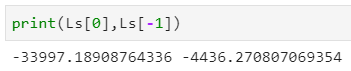
\includegraphics[width=1\linewidth]{img/final_0.PNG}
        \caption{$\texttt{random\_seed}=0$}\vspace{2mm}
    \end{subfigure}
    \begin{subfigure}[H]{0.5\textwidth}
        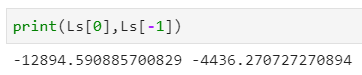
\includegraphics[width=1\linewidth]{img/final_1.PNG}
        \caption{$\texttt{random\_seed}=1$}\vspace{2mm}
    \end{subfigure}
    \begin{subfigure}[H]{0.5\textwidth}
        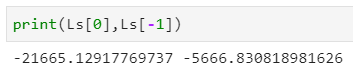
\includegraphics[width=1\linewidth]{img/final_42.PNG}
        \caption{$\texttt{random\_seed}=42$}
    \end{subfigure}
    \begin{subfigure}[H]{0.5\textwidth}
        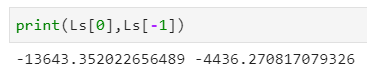
\includegraphics[width=1\linewidth]{img/final_777.PNG}
        \caption{$\texttt{random\_seed}=777$}
    \end{subfigure}
    \caption{The first(left) and last(right) log-likelihood values}
    \label{fig1}
\end{figure}
Fig. \ref{fig1} and \ref{fig2} are the results. The results show that the EM algorithm is sensitive with respect to the initialization. It is quite interesting that the algorithm reached to the almost same value with \texttt{random\_seed} of 0, 1 and 777. However, when \texttt{random\_seed} is 42, the algorithm converged to very different value. Also, it took 10 times more iterations to converge, which looks quite wrong.
\begin{figure}[H]
    \begin{subfigure}[H]{0.5\textwidth}
        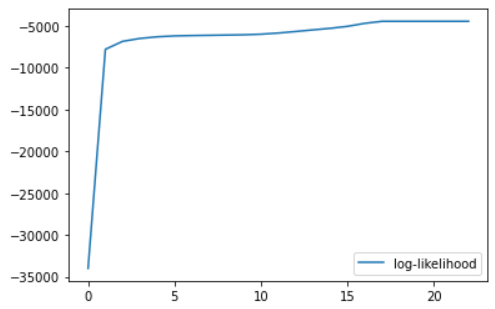
\includegraphics[width=1\linewidth]{img/plot_0.PNG}
        \caption{$\texttt{random\_seed}=0$}\vspace{2mm}
    \end{subfigure}
    \begin{subfigure}[H]{0.5\textwidth}
        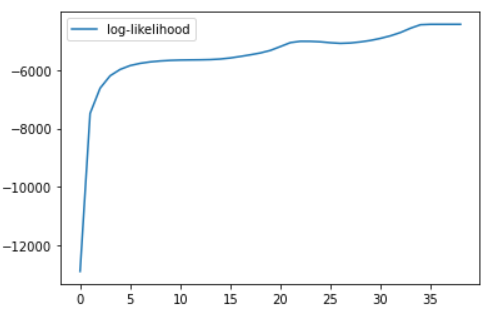
\includegraphics[width=1\linewidth]{img/plot_1.PNG}
        \caption{$\texttt{random\_seed}=1$}\vspace{2mm}
    \end{subfigure}
    \begin{subfigure}[H]{0.5\textwidth}
        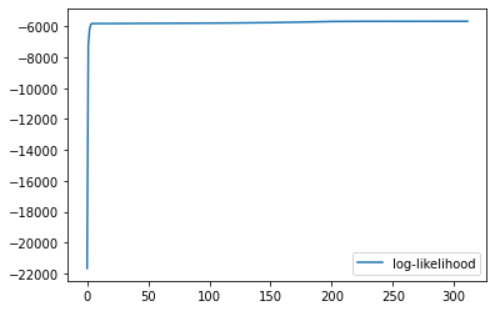
\includegraphics[width=1\linewidth]{img/plot_42.PNG}
        \caption{$\texttt{random\_seed}=42$}
    \end{subfigure}
    \begin{subfigure}[H]{0.5\textwidth}
        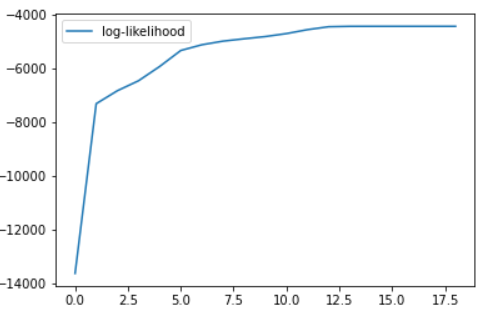
\includegraphics[width=1\linewidth]{img/plot_777.PNG}
        \caption{$\texttt{random\_seed}=777$}
    \end{subfigure}
    \caption{The trace plot of the log-likelihood}
    \label{fig2}
\end{figure}
\end{document}
